\documentclass[12pt]{article}
\usepackage{graphicx}
\usepackage{fullpage}
\usepackage{float}
\usepackage[symbol]{footmisc}
\graphicspath{{../images/}}
\usepackage{titlesec}% http://ctan.org/pkg/titlesec
\titleformat{\section}%
  [hang]% <shape>
  {\normalfont\bfseries\Large}% <format>
  {}% <label>
  {0pt}% <sep>
  {}% <before code>
\renewcommand{\thesection}{}% Remove section references...
\renewcommand{\thesubsection}{\arabic{subsection}}%... from subsections

\title{Radio Interferometry}
\author {
Kevin Yu
}

\begin{document}
\maketitle

\begin{abstract}
Radio interferometry allows us to.  We use a radio interferometer to observe the Sun, the Moon, and (point source). We measure the East-West baseline of our interferometer to be $10.06$ m. We use a similar method to determine that the declination of 3C144 is $blah$, close to the computed value of $bleh$. Finally, we approximate the angular diameter of the Sun and the Moon.
\end{abstract}

\section{Introduction}
We can use interferometry for various purposes

In the first section, we discuss the equipment being used and how interferometry works (basically) and taking the correlaetion.

In the next section, we discuss the fringe pattern.

In the next section, we will discuss how we choose sources and how we locate them in the sky. (Rotation matricies and such)

In the next section, we discuss methods of using an observation of a point source to measure its declination, by fitting the fringe pattern. This includes fourier filtering and methods of least squares fitting. 

In the next section, we discuss how a non-point source forces us to integrate the fringe pattern over the source.

Finally, we will use that to meausure the angular diameters of the sun and the moon. This includes how we find the zero crossings of the observational data, and how we vary R in the theoretical bessel function to minimzie the deviation between our zero crossings and the observaitons.

\section{The Interferometer}
The interferometer consists of two radio dishes separated along an approximately East-West baseline. The baseline separation between the two dishes is approximately $B_y = 10$ m. We observe radiation at $\lambda = 2.75$ cm wavelengths.

Interferometry depends on the time-delay between the detection of a plane wave at each receiver. This time-delay $\tau$ varies as the source moves across the sky and is dependent on a couple factors: the geometrical difference in distance between the two detectors and the speed of light, $c$.

Because we are on a E-W baseline, our geometrical time-delay is described by this expression:
\begin{equation}
\tau_g= \left( \frac{B_y}{c} \right) \cos{\delta} \cos{h_a}
\end{equation}
in which $B_y$ is the baseline distance, $\delta$ is the declination of the object, and $h_a$ is the hour-angle of the object\footnote{This is a time-like coordinate, equal to the observer's local sidereal time minus the object's right ascension.}.

The output of the interferometer is the time average of the product of the signals received at each detector. When they are correlated and time averaged, the amplitude we observe is described by the following:
\begin{equation}
F(h_a) = \cos(2\pi \nu [\tau_g (h_a) + \tau_c]) \label{eq:fringe-output}
\end{equation}.

In the above expression, $\tau_c$ is the cable delay. The voltage we detect should be described by this expression (CITE lab manual).
\begin{equation}
F(h_a) = \cos{2\pi \nu \tau_c} \cos{\left( 2\pi \frac{B}{\lambda} 
\cos{\delta} \sin{h_a} \right)} - \sin{2\pi \nu \tau_c} \sin{\left( 2\pi \frac{B}{\lambda} 
\cos{\delta} \sin{h_a} \right)} \label{eq:fringe-amplitude}
\end{equation}
In Eq. \ref{eq:fringe-amplitude}, $\lambda$ is the wavelength of the radiation we are observing and $\nu$ is the frequency. 

This descibes a sinusoidal ``fringe pattern" whose frequency varies as the hour-angle (and declination) of the source changes. This can be applied to point sources, from which we essentially are detecting plane waves from a single location in the sky.

This equation is more suited than Eq. [the other one]  to the least squares fitting method that we will employ in Section X, in which we will fit the constant coeffecients $ \cos{2\pi \nu \tau_c}$ and $ \sin{2\pi \nu \tau_c}$.

The local fringe frequency at a particular declination and hour angle is:
\begin{equation}
f_f(h_a) = \frac{B}{\lambda} \cos{\delta} \cos{h_a} \label{eq:local-fringe-frequency}
\end{equation}

\subsection{Locating Objects}
The coordinates of celestial bodies are most often given in the coordinates of right ascension (RA) and declination (DEC). Right ascension is the object's angular distance eastward relative to the vernal equniox. Declination is the angle between the object and an axis parallel to the Earth's north pole. The are Earth based coordinates, meaning they do not change depending on one's location on Earth. However, they are not that useful to an observer who wants to track the object's motion as it travels across the sky.

To know where to point the telescope, we must translate our coordinates into altitude and azimuth, which represent a position on the sky relative to the observer. Altitude of $90^\circ$ is directly overhead, while altitude of $0^\circ$ is on the horizon. Azimuth represents what direction the source is relative to North, and is often represented in hours (0 hours is directly north, while 12 hours is directly south).

To transform from (RA, DEC) to (AZ, ALT), we first want to convert from (RA, DEC) to (HA, DEC). HA, or hour angle, is the difference between the observer's local sidereal time and the object's right ascension. The local sidereal time increases linearly and thus the hour angle is a time-like coordinate that describes the object's angular position relative to the observer rather than the vernal equniox.

From (HA, DEC), we can apply rotations based on the observer's latitude and longitude to rotate the coordinates to (AZ, ALT). These transformations are essential to finding the location objects in the night sky.

Another thing to note is that because the Earth precesses slowly, the ``Earth based" coordinates of RA and DEC will start to change over the years. Thus, right ascensions and declinations are recorded along with their \textit{epoch}, which allow a reference point from which the coordinates can be precessed.

In this lab, we will primarily use the Python module PyEphem, which handles such conversions and precessions with ease.
\subsection{Observation Targets}
[include a table of objects]
The objects that we will observe. We will observe 3C144, the Crab Nebula, which is a point source for our interferometer, in order to deduce values for our baseline $B_y$ and to measure the source's declinaion. Furthermore, we observe the Sun and Moon in attempts to measure their angular diameter using interferometery.


\subsection{Tracking Objects Using Interferometer}
Homing, repointing frequency
Original measurements of both point source data and the Sun provided very ungood results. We suspected that this was due to a low repointing frequency. We originally pointed once every 2 minutes. According to Karto, the apeture is what. That means the object will move out of the apeture within four minutes. 



\subsection{Measurments using 3C144}
Determinations of certain quantities can be determined by fitting Eq. \ref{eq:fringe-amplitude} to data from 3C144. This equation has three unknown quantities: the time delay due to differences in cable length, $\tau_c$, the baseline $B_y$, and the declination of the target, $\delta$. As we will see, if we assume our value of $\delta$ is accurate (as looked up in a catalog) we can use least squares fitting to determine our baseline $B_y$. Similarly, assuming a value for the baseline $B_y$, we can use a similar procedure to determine the actual declination of 3C144.

\subsubsection{Processing 3C144 Data}

\begin{figure}[H]
\center{
  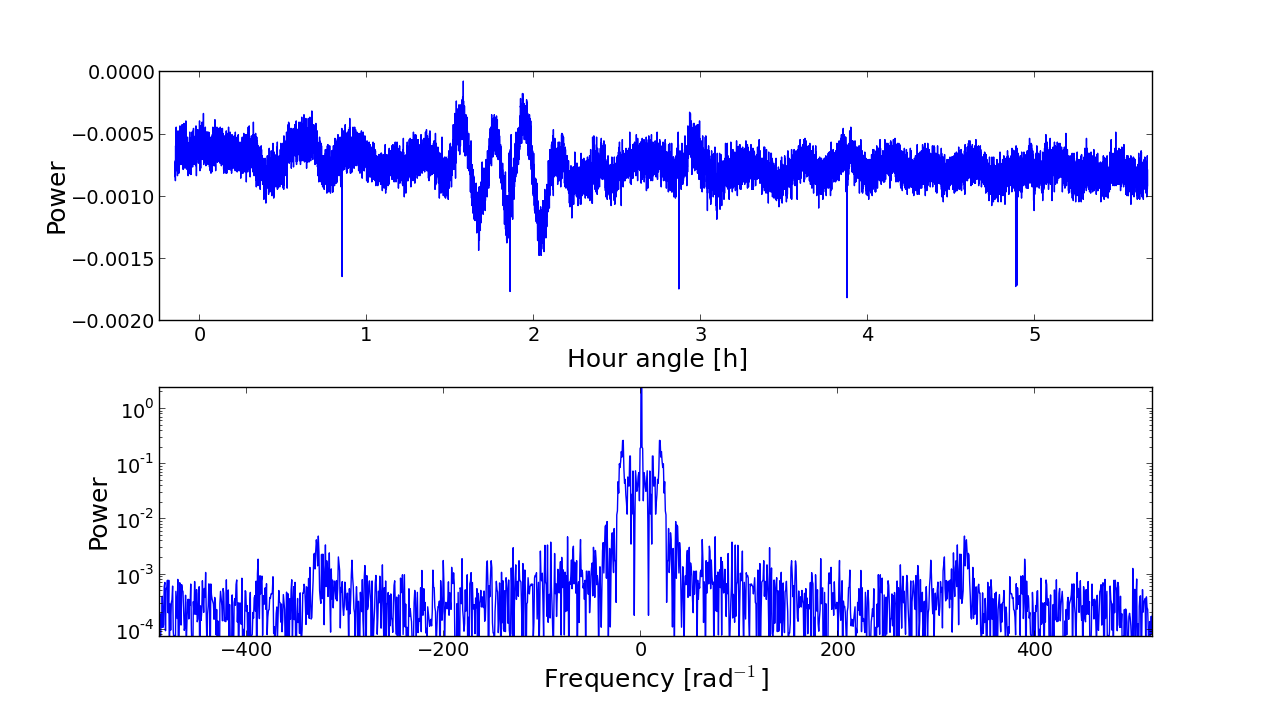
\includegraphics[width=440px]{original}
}
\caption[SODUMB]{Interferometric data taken for 3C144 on 4/3/2014. Data collection began just before 3C144 crossed the meridian.}
\label{fig:original}
\end{figure}

Figure \ref{fig:original} shows the signal collected for just about half of 3C144's transit across the sky. The data contains a lot of noise and has large, low frequency features that are inconsistent with the expected shape of the fringe; from Eq. \ref{eq:fringe-output}, the signal should simply be a sinusoidal wave of about constant amplitude and varying frequency. Additionally, there is a clear DC component to the signal. These components of our signal must be removed before fitting can be done.

To extract the signal we are interested in, we first will use the technique of Fourier Filtering to eliminate frequencies which we know should not be seen in the 3C144 signal. We can remove frequencies by transforming to the frequency domain, eliminating unwanted frequencies, and then applying an inverse fourier transform back into the time domain.

The frequency range which we will attempt to extract will be determined by the range of fringe frequencies we expect by Eq. \ref{eq:local-fringe-frequency}. The fringe frequency reaches a maximum value where $|\cos{\delta} \cos{h_a}|$ is a maximum. The same reasoning applies to the minimum fringe frequency. For our observation of 3C144, these extrema occur at the following fringe frequencies:
\begin{eqnarray}
f_{f, max} = 371\ rad^{-1}\\
f_{f, min} = 32\ rad^{-1}
\end{eqnarray}
We apply a bandpass Fourier filter to our data that removes frequency components less than $f_{f, min}$ and greater than $f_{f, max}$. The resulting signal and its power spectrum are shown in Figure \ref{fig:filtered}.

Because the function that we will be fitting to can be written as Eq. \ref{eq:fringe-output}, the main goal of fitting here is to fit $\delta$ or $B_y$ such that the fringe frequency matches the data. However, it is clear from Figure \ref{fig:filtered} that our fringe contains modulations in amplitude. This causes a problem in least-squares fitting as the amplitude modulations will artificially weight certain sections of the data more strongly than others; in particular, sections of data with a smaller amplitude will have their residuals automatically smaller. 

We solve this issue by normalizing the data in bins of 200 data points to the maximum value in each bin. Though this could amplify noise more in some sections of the data than others, the overall result should be that minimizing the square of the residuals will allow us to find the best fit fringe frequency. Using this technique of normalizing to the amplitude of nearby points turns out to be extremely important in successfully fitting a the fringe amplitude to the data, and allows us to make good meaurements of both our interferometer's baseline and the declination of 3C144.

\begin{figure}[H]
\center{
  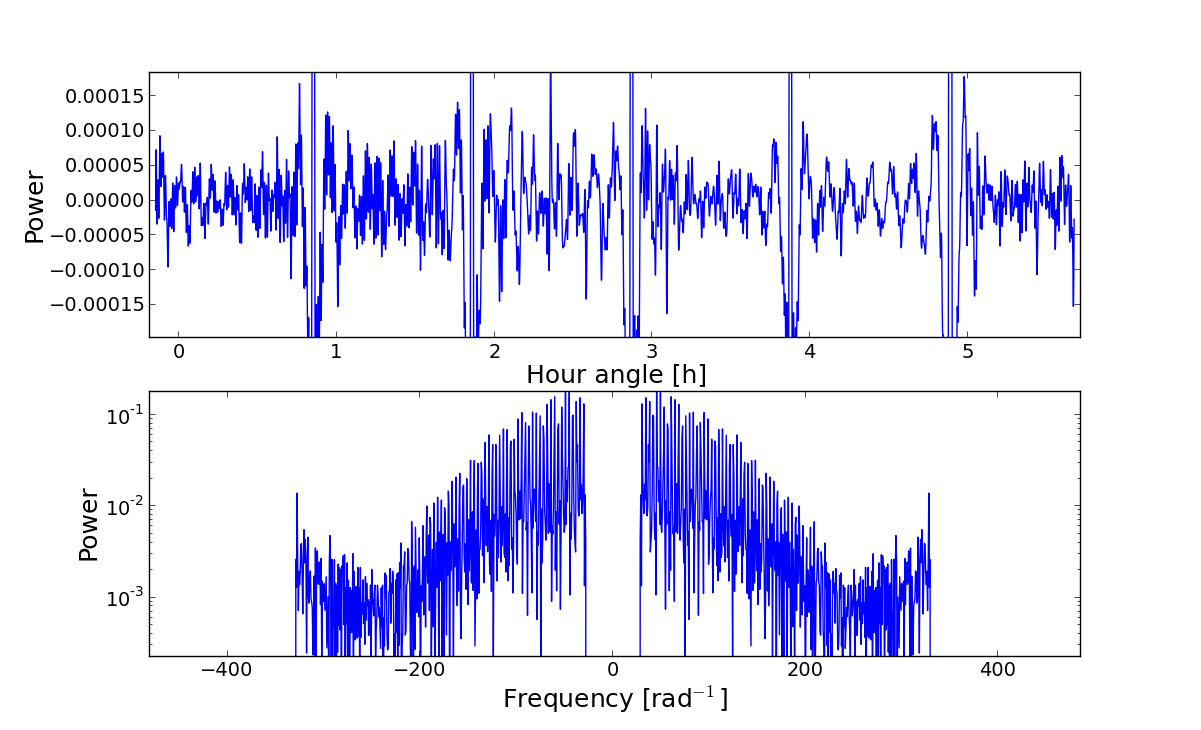
\includegraphics[width=440px]{filtered}
}
\caption[SODUMB]{Data for 3C144 after filtering out frequencies greater than the maximum fringe frequency and slower than the minimum fringe frequency. The DC offset is removed. Spikes at each hour occur due to homing of the telescope and may have been exaggerated by the normalization methods used.}
\label{fig:filtered}
\end{figure}

\subsubsection{Fitting the Baseline}
For purposes of determining the baseline using 3C144, we use the documented declination of $\delta_{J2000} = 22^\circ 00'52.1'' = 0.3842$ rad. The precessed value of this declination in the current epoch is $\delta_{J2000} = 22^\circ 04'14'' = 0.3852$ rad.

A least squares method can be used on the filtered and normalized data shown in Figure [filtered and normalized]. The method we use to fit the baseline is as follows:

\begin{enumerate}
  \item We rewrite Eq. \ref{eq:fringe-amplitude} with constant coefficients filled in for the $\tau_c$ dependent factors. 
  \begin{equation}
F(h_a) = C_1 \cos{\left( 2\pi \frac{B_y}{\lambda} 
\cos{\delta} \sin{h_a} \right)} - C_2 \sin{\left( 2\pi \frac{B_y}{\lambda} 
\cos{\delta} \sin{h_a} \right)} \label{eq:fringe-amplitude}
\end{equation}

  \item To fit $B_y$, we iterate over a range of possible baseline values and apply a linear least-squares fit using each one. From the lab manual, we know that the baseline is near $10$ m; however, we probe values of $B_y$ ranging from $1.00$ m to $20.00$ m in order to demonstrate the efficacy of this method. We try values of $B_y$ in steps of $0.01$ m; this step size will limit the resolution at which we can determine the baseline.
   \item We look at the $\chi^2$ values for each of the linear fits performed in the last step. The baseline value corresponding to the smallest value of $\chi^2$ is our best fit baseline.
\end{enumerate}

\begin{figure}[H]
\center{
  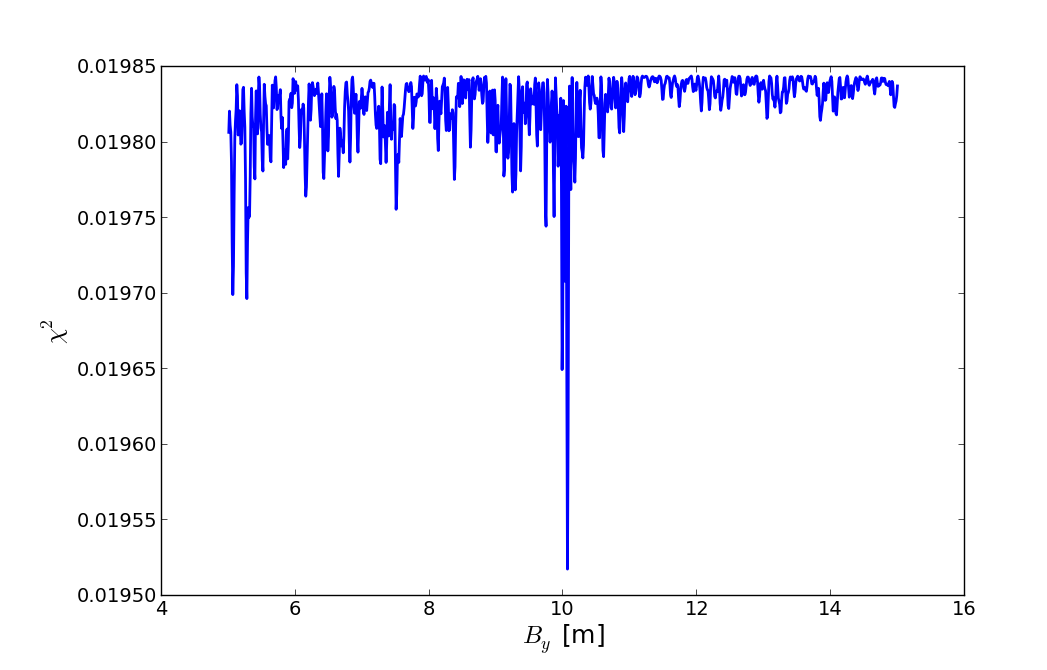
\includegraphics[width=380px]{baseline_chi2}
}
\caption[SODUMB]{The $\chi^2$ values of linear fits for various values of $B_y$. The $\chi^2$ value, which is defined as the sum of the squared residuals between the fit and the observations, divided by the degrees of freedom in each fit. It is minimized at $B_y=10.06$ m.}
\label{fig:baseline-chi2}
\end{figure}

By applying the above procedure, we find a range of $\chi^2$ plotted in Figure \ref{fig:baseline-chi2}. There is a single point that clearly minimizes the $\chi^2$ of the fit; this is our measurement of the baseline:
\begin{equation}
B_y = 10.06\ m 
\end{equation}
Before moving on, allow me to point out the importance of normalizing the data. Without normalizing the data and leaving the amplitude fluctuations, the array of $\chi^2$ for the very same baseline values appears as in Figure. \ref{fig:bad-chi2}. Not only is the measurement of $B_y$ significantly off, there are also many comparable local minima which leaves a lot of uncertainty as to the true value of $B_y$.

\begin{figure}[H]
\center{
  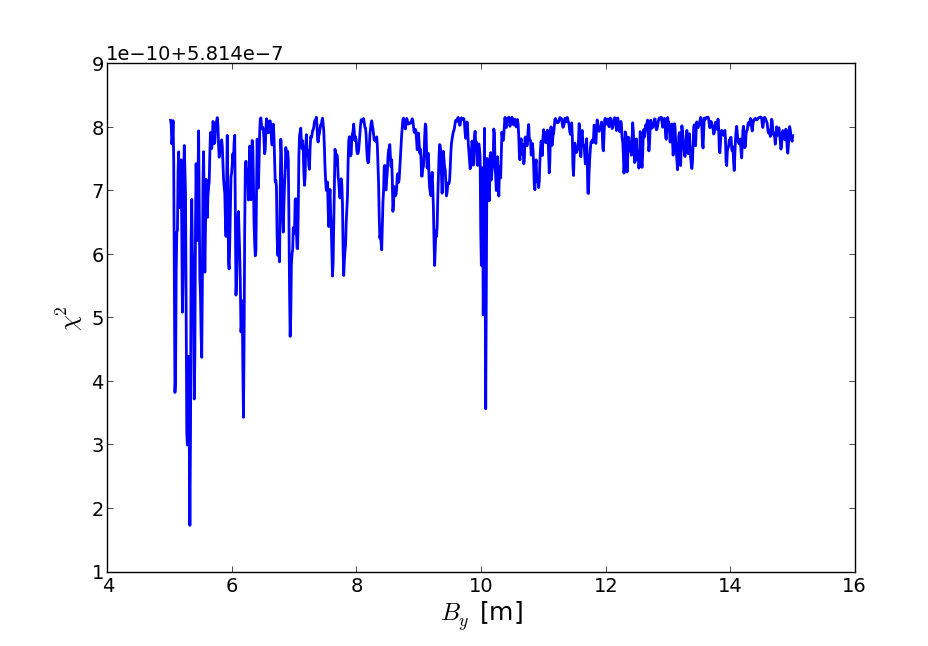
\includegraphics[width=380px]{bad_chi2}
}
\caption[SODUMB]{The $\chi^2$ values of linear fits for various values of $B_y$, using unfiltered and unnormalized data. There is a local minima at $B_y=10.06$ m, but due to noise and other contributions, there are many comparable spikes in $\chi^2$ and in fact is minimzed in this range by $B_y \approx 5.3$ m. It is clear that filtering and normalization was necessary to properly fit the data.}
\label{fig:bad-chi2}
\end{figure}

\subsection{Declination of 3C144 (Crab Nebula)}
We will now take the baseline length of $B_y = 10.06$ m as a truth of reality and will fit the declination using the same method as above. Instead of probing different baseline values, we probe different values of the declination to minimize the square residuals.

Knowing that the declination should be around $22^\circ$, we will try values of $\delta$ from $12.00^\circ$ to $32.00^\circ$ in steps of $0.01^\circ$. The $\chi^2$ values for these declinations are shown in Figure [chi2 for dec] and the best fit value for the declination is:
\begin{equation}
\delta_{3C144} = 22^\circ 14'39.1''
\end{equation}
This measurement is reasonably close to the PyEphem calculated value of $\delta_{J2000} = 22^\circ 04'14'' $; it is off by less than $0.2^\circ$. 

\begin{figure}[H]
\center{
  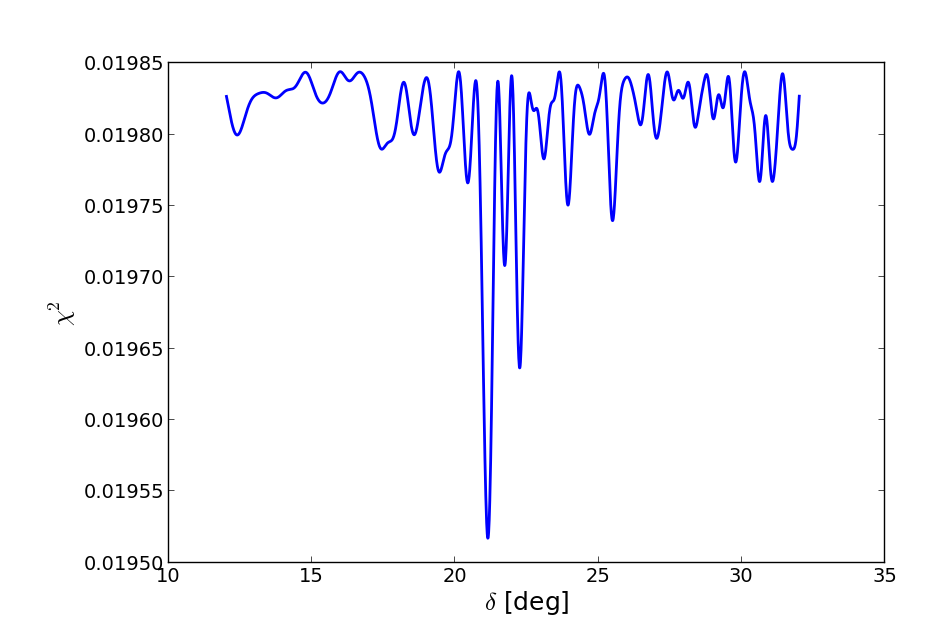
\includegraphics[width=380px]{dec_chi2}
}
\caption[SODUMB]{The $\chi^2$ values of linear fits for various values of $\delta$, using the same method as for the baseline. The $\chi^2$ value is minimized for $\delta = 22.24^\circ$. There is a bit of uncertainty here due to the fact that another value of $\delta$ near $23^\circ$ has a comparable local minima in $\chi^2$.}
\label{fig:dec-chi2}
\end{figure}

\subsection{The Sun}
Sources whose brightness span an angle in the sky (i.e. not point sources) contain additional information in the fringe amplitude. The data collected is the integral of the entire object multipled by the fringe amplitude. As we know, the interferometric data collected in the u-v plane is the fourier transform of the true sky.

The Sun's intensity as a function of angular separation from its center can be described by the following equation:
\begin{equation}
I(\delta h ) = \frac{(R^2 - \Delta{h}^2)^{1/2}}{R}
\end{equation}
If we integrate this intensity over the fringe, we find that the modulating function is
\begin{equation}
MF_{theory} = \frac{1}{R} \int_{-R}^{R} (R^2 - \Delta{h}^2)^{1/2} \cos{(2\pi f_f \Delta{h})} d\Delta{h}
\end{equation}
In order to evaluate the integral numerically, we rewrite this as a summation:
\begin{equation}
MF_{theory} \approx \sum_{n=-N}^{n=+N} \left[ 1- \left( \frac{n}{N} \right) ^2 \right]^{1/2} \cos{\frac{2\pi f_f R n}{N}}
\end{equation}  
It looks a little something like this.

\begin{figure}[H]
\center{
  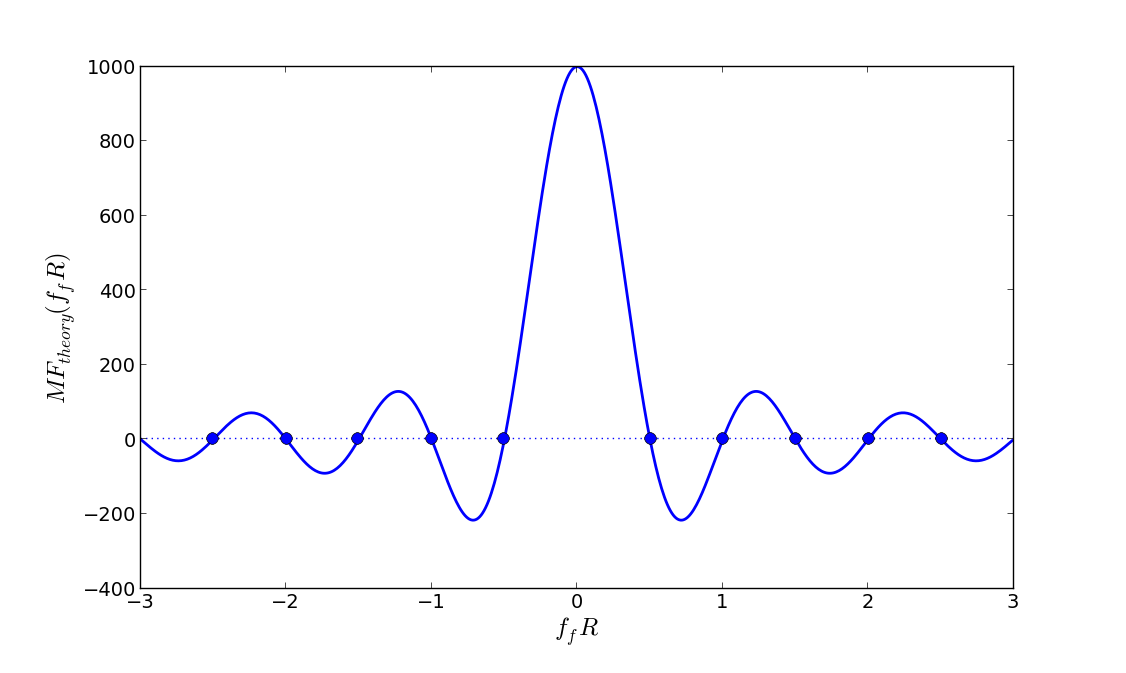
\includegraphics[width=440px]{MF}
}
\caption[SODUMB]{Theoretical modulating bessel function.}
\label{fig:MF}
\end{figure}

\subsubsection{Measuring Solar Diameter}
The Sun's intensity allows our signal to generally overwhelm the noise of the system. The shape of the bessel-function envelope can already be seen even in the unreduced dataset (Figure [unreduced solar]).

Similar, to the data for 3C144, we can determine the highest fringe frequency we expect and filter out noise higher than that frequency. Addiitonally, we can apply a filter by which we divide the data into bins and subtract the mean of each bin off data points in the bin. This will help center some sections of the data on zero without damaging the overall shape of the envelope,which is important in determining the angular radius of the sun. 

To determine the angular diameter of the Sun, we note that the theoretical $MF$ is a function of the quantity $f_f R$, and has zero crossings at certain values as shown in Figure [theoretical MF]. These roots of this function are as follows:
\begin{equation}
f_f R = [ \ 0.60975\  1.11675\  1.61925 \ 2.12075\  2.62125\ \ldots\ ] \label{eq:fRs}
\end{equation}
Here's the gameplan: if we extract the envelope of our data and find its minima, the hour angle $h_a$ at which the envelope reaches a minimum corresponds to the zero's of the bessel function. At these values of $h_a$, we can compute the corresponding local fringe frequencies using Eq. \ref{eq:local-fringe-frequency}. By using a fringe frequnecy at which we observe a minima in the envelope, we can divide the values in Eq. \ref{eq:fRs} by that fringe frequency to get the possible values of $R$.

To determine the aforementioned values of $h_a$, we begin by extacting the envelope. To do this, we divide the dataset into bins of 50 data points each replace each bin with a point equal to the maximum of the absolute value of points in the bin. As long as the size of the bins is small enough to preserve the overall shape and features of the envelope, but large enough to span at least one period of the fringe, the resulting data points will represent the envelope with the proper magnitude. The result of this envelope detection method is shown in Figure [solar envelope].

By inspecting the shape of the envelope, we see minima marked by the circles in the plot. At each one, we can take a small slice of the envelope and fit a second order polynomial to the region. The minimal value of this fitted polynomial is is the hour angle of the zero crossing.

As we can see from Figure [zoom in on all 4 zero crossings individually]
the crossings closer to the center are not very well defined and the location that they hit their minima is iffy. In contrast, the crossings further out are more clearly defined, so I will begin by using those\footnote{I will go back to the first crossing later and we find that it raises some questions.}. The exterma for these two polynomials occur at $-3.214$ h and at $3.238$ h; reassuringly symmetric about the meridian. The corresponding fringe frequencies determined using Eq. \ref{eq:local-fringe-frequency} are listed in the following table, as well as the values of $R$ that allow that zero crossing using Eq. \ref{eq:fRs}:
\begin{table}
\begin{center}
  \begin{tabular}{c | c | c }
    $h_a$ [h] & $f_f$ [rad$^{-1}$] & Possible $R$ [deg]\\ \hline
    -3.214 & 237.345 & [ 0.147  0.270  0.391  0.512  ... ] \\
    3.238 & 235.643 &  [ 0.148  0.272  0.394  0.515  ... ] \\
    \end{tabular}
\end{center}
\caption{Values of R that give an angular diameter of greater than $1^\circ$ can be ignored because that is approximately the limit of our telescope's apeture.}
\label{tbl:firfrequencies}
\end{table}

If we assume that these zero crossings correspond to the second zero crossings in Figure [theoretical MF], then our result (averaging the two values of R in the above table) is:
\begin{equation}
D = 2R = 0.542^\circ \nonumber
\end{equation}

However, assuming this is the second zero crossing is a bit problematic because it requires two more zero crossings (one positive, one negative) closer to zero. As we saw in Figure [the zero crossings], these local minima in the envelope are not as well defined and it is harder to determine at what hour angle they occur at. However, by fitting a second order polynomial to these regions, we find that minima occur at roughly $-2.312$ h and $2.476$ h. However, assuming these correspond to the smallest roots of $MF$, the corresponding diameter measurements are $D = 0.239^\circ$ and $D = 0.246^\circ$, which are a factor of two off of the actual value.

Thus it is hard to confidently say that the measurement of $D = 0.542^\circ$ is totally valid, due to the missing node predicted $MF_{theory}$. It is possible that the other node is removed due to contributions from asymmetric contributions of the sun as it crosses the meridian.

I might investigate why they are so far off and if adjustmenets in $h_a$ for that minima changes the location of the minima at all. 

\subsection{The Moon}
If I wasn't so late, I'd probably try analyzing the moon data too.

\section{Conclusion}


\section{Acknowledgement}


\end{document}